\documentclass[14pt,a4paper]{extarticle}

\usepackage[utf8]{inputenc}
\usepackage[T2A]{fontenc}
\usepackage[russian]{babel}
\usepackage{geometry}
\usepackage{listings}
\usepackage{graphicx}
\usepackage{tabularx}
\usepackage{booktabs}
\usepackage{longtable}
\usepackage{array}
\usepackage{float}
\usepackage{xcolor}
\usepackage{caption}
\usepackage{hyperref}

\geometry{left=30mm,right=15mm,top=20mm,bottom=20mm}
\graphicspath{{../screens/}}
\hypersetup{colorlinks=true, linkcolor=black, urlcolor=blue}

\definecolor{codebg}{RGB}{246,248,250}
\definecolor{codeborder}{RGB}{208,215,222}
\definecolor{rubyred}{RGB}{160,32,32}
\definecolor{commentgray}{RGB}{100,116,139}

\lstdefinelanguage{RubyCustom}{
  language=Ruby,
  morekeywords={before_action,helper_method,belongs_to,has_many,validates,namespace,scope,resource,render,redirect_to,send_data},
  sensitive=true
}

\lstdefinelanguage{JavaScriptCustom}{
  keywords={const,let,var,function,return,if,else,await,async,document,fetch,JSON,new},
  keywordstyle=\bfseries\color{rubyred},
  ndkeywords={class,export,import,from},
  ndkeywordstyle=\bfseries\color{blue},
  identifierstyle=\color{black},
  sensitive=true,
  comment=[l]{//},
  morecomment=[s]{/*}{*/},
  commentstyle=\color{commentgray}\ttfamily,
  stringstyle=\color{teal}
}

\lstset{
  basicstyle=\ttfamily\small,
  backgroundcolor=\color{codebg},
  frame=single,
  rulecolor=\color{codeborder},
  numbers=left,
  numberstyle=\tiny\color{commentgray},
  breaklines=true,
  tabsize=2,
  showstringspaces=false,
  keywordstyle=\bfseries\color{rubyred},
  commentstyle=\color{commentgray},
  stringstyle=\color{teal},
  captionpos=b
}

\title{Курсовой проект по дисциплине «Методики разработки современных WEB-приложений»\\
\large Разработка WEB-приложения на Ruby on Rails}
\author{Татарченко Андрей Александрович, группа 5140903/50401}
\date{Санкт-Петербург, 2026}

\begin{document}

\begin{titlepage}
\begin{center}
Санкт-Петербургский политехнический университет Петра Великого\\
Институт компьютерных наук и кибербезопасности\\
Высшая школа прикладной информатики

\vfill

{\Large КУРСОВОЙ ПРОЕКТ}\\[1.2cm]
{\Large Разработка WEB-приложения на Ruby on Rails}\\[0.4cm]
по дисциплине «Методики разработки современных WEB-приложений»

\vfill

\begin{flushright}
Выполнил\\
студент гр. 5140903/50401\\
\textbf{Татарченко Андрей Александрович}\\[0.7cm]
Преподаватель\\
доцент, к.т.н.\\
\textbf{Иванищев Алексей Вячеславович}
\end{flushright}

\vfill

Санкт-Петербург\\
2026
\end{center}
\end{titlepage}

\newpage
\section*{Задание на выполнение курсового проекта}

Студенту: \textbf{Татарченко Андрей Александрович}. Группа: \textbf{5140903/50401}.

\begin{enumerate}
  \item Тема курсового проекта: разработка WEB-приложения на Ruby on Rails.
  \item Срок сдачи студентом законченной работы: 25.05.2026.
  \item Исходные данные к работе: требования дисциплины, документация Ruby on Rails 8, PostgreSQL, Active Record, I18n, Fetch API, материалы практических занятий и локально разработанное приложение MallExpert SPb.
  \item Содержание пояснительной записки: введение; постановка задачи; выбор технологий; проектирование MVC-приложения и базы данных; реализация авторизации, API, интерфейса, локализации и CSV-экспорта; тестирование; запуск; результаты; заключение; список источников; приложения.
  \item Перечень графического материала: схема базы данных, схема пользовательского сценария, скриншоты интерфейса, листинги ключевых файлов.
  \item Консультанты: доцент, к.т.н. Иванищев Алексей Вячеславович.
\end{enumerate}

Дата получения задания: 03.02.2026.

\vspace{1cm}
\begin{tabularx}{\textwidth}{X X}
Преподаватель \newline \newline \rule{55mm}{0.4pt} / А.В. Иванищев / &
Задание принял к исполнению \newline \newline \rule{55mm}{0.4pt} / А.А. Татарченко /
\end{tabularx}

\newpage
\section*{Аннотация}

В курсовом проекте я разработал WEB-приложение \textbf{MallExpert SPb} на Ruby on Rails 8 и PostgreSQL. Приложение предназначено для экспертной оценки торговых центров Санкт-Петербурга. Пользователь регистрируется, входит в систему, выбирает категорию ТЦ, получает первую неоцененную карточку, выставляет оценку плавным ползунком от 1 до 100 и оставляет текстовый комментарий.

Я реализовал ручную сессионную авторизацию через \texttt{has\_secure\_password}, \texttt{bcrypt}, \texttt{SessionsController} и \texttt{session[:user\_id]}. Для динамического интерфейса я написал JavaScript-модуль на Fetch API, который получает карточки и сохраняет оценки без полной перезагрузки страницы. Также мной реализованы RU/EN-локализация, личный кабинет, расчет средней оценки и экспорт пользовательских данных в CSV.

\tableofcontents
\newpage

\section{Введение}
\subsection{Актуальность}

В современных WEB-приложениях пользователь часто не просто просматривает объекты, а принимает решение на основе персональной или экспертной оценки. Я выбрал эту модель для курсового проекта, потому что она позволяет показать полный цикл разработки: хранение пользователей, предметные справочники, персональные оценки, API, клиентскую динамику и отчетность.

Предметной областью я выбрал торговые центры Санкт-Петербурга. Такой объект оценки понятен пользователю: можно сравнивать расположение, формат досуга, масштаб комплекса, семейную инфраструктуру и общее впечатление от посещения. В отличие от абстрактных изображений, ТЦ имеют практическую ценность и хорошо подходят для демонстрации экспертной системы выбора.

Отдельно я сделал UX-акцент на шкале от 1 до 100. Шкала 1--5 удобна для грубого отзыва, но экспертная оценка требует большей точности. Поэтому в моем приложении используется интерактивный HTML5 range-ползунок, похожий по ощущению на стикеры-опросы в социальных сетях.

\subsection{Цель и задачи}

Цель моей работы - разработать WEB-приложение MallExpert SPb на Ruby on Rails 8 и PostgreSQL для экспертной оценки торговых центров Санкт-Петербурга.

Для достижения цели я выполнил следующие задачи:
\begin{itemize}
  \item спроектировал структуру Rails-приложения;
  \item разработал модели \texttt{User}, \texttt{Theme}, \texttt{MallItem}, \texttt{Evaluation};
  \item реализовал ручную авторизацию через \texttt{has\_secure\_password};
  \item настроил маршруты с локализацией \texttt{/:locale};
  \item разработал JSON API для получения ТЦ и сохранения оценки;
  \item написал клиентский JavaScript на Fetch API;
  \item реализовал личный кабинет и CSV-экспорт;
  \item добавил сиды на 10 реальных ТЦ Санкт-Петербурга;
  \item написал unit и integration-тесты;
  \item подготовил Dockerfile, скриншоты и итоговый отчет.
\end{itemize}

\subsection{Краткое описание проекта}

MallExpert SPb работает как цикл оценки. Пользователь входит в систему, выбирает категорию, получает карточку торгового центра и ставит оценку. После сохранения сервер выдает следующий неоцененный объект. Когда в категории заканчиваются неоцененные ТЦ, пользователь получает сообщение о завершении.

\section{Постановка задачи и требования}
\subsection{Функциональные требования}

\begin{longtable}{|p{7mm}|p{62mm}|p{70mm}|}
\hline
N & Требование & Реализация \\ \hline
1 & Регистрация пользователя & \texttt{UsersController}, модель \texttt{User}, \texttt{bcrypt} \\ \hline
2 & Вход и выход & \texttt{SessionsController}, \texttt{session[:user\_id]} \\ \hline
3 & Защита рабочей области & \texttt{ApplicationController\#authorize} \\ \hline
4 & Выбор категории ТЦ & модель \texttt{Theme}, HTML select \\ \hline
5 & Выдача первого неоцененного ТЦ & \texttt{MallsApiController\#index} \\ \hline
6 & Оценка 1--100 & \texttt{input type=range}, модель \texttt{Evaluation} \\ \hline
7 & Комментарий к оценке & поле \texttt{comment} \\ \hline
8 & Асинхронное сохранение & JavaScript \texttt{fetch()} \\ \hline
9 & Личный кабинет & \texttt{ProfilesController\#show} \\ \hline
10 & CSV-экспорт & \texttt{ProfilesController\#export}, \texttt{Evaluation.to\_csv} \\ \hline
11 & RU/EN интерфейс & \texttt{config/locales/ru.yml}, \texttt{config/locales/en.yml} \\ \hline
\end{longtable}

\subsection{Нефункциональные требования}

Я заложил требования к надежности, безопасности, удобству и воспроизводимости. Пароли не хранятся в открытом виде. Критичные ограничения продублированы на уровне Active Record и PostgreSQL. Основной сценарий оценки работает без перезагрузки страницы. Проект можно запустить локально или через Docker.

\section{Выбор технологий и инструментов}

Ruby on Rails 8 я выбрал из-за зрелой MVC-архитектуры, удобной маршрутизации, Active Record, миграций, ERB-шаблонов, сессий, I18n и встроенных тестов. PostgreSQL я использовал как надежную СУБД с внешними ключами, уникальными индексами и check constraints.

\begin{table}[H]
\centering
\begin{tabularx}{\textwidth}{lX}
\toprule
Компонент & Назначение \\
\midrule
Ruby 3.3.11 & язык серверной разработки \\
Ruby on Rails 8 & MVC-фреймворк \\
PostgreSQL 16 & хранение данных \\
Active Record & ORM, миграции, связи и валидации \\
bcrypt & безопасное хранение паролей \\
Vanilla JS + Fetch API & асинхронный интерфейс \\
I18n & локализация RU/EN \\
Minitest & тестирование моделей и сценариев \\
Docker & переносимый запуск \\
\bottomrule
\end{tabularx}
\end{table}

\section{Проектирование}
\subsection{Архитектура MVC}

Я разделил приложение на стандартные Rails-слои. Модели отвечают за данные и правила, контроллеры - за обработку запросов, представления - за HTML-интерфейс, а JavaScript - за динамический рабочий сценарий. Для JSON-взаимодействия я вынес отдельный namespace \texttt{/api/v1}.

\subsection{Маршрутизация}

\begin{table}[H]
\centering
\begin{tabularx}{\textwidth}{l l l X}
\toprule
URL & Метод & Контроллер & Назначение \\
\midrule
\texttt{/ru} & GET & \texttt{MallsController#index} & рабочая область \\
\texttt{/ru/signup} & GET/POST & \texttt{UsersController} & регистрация \\
\texttt{/ru/login} & GET/POST & \texttt{SessionsController} & вход \\
\texttt{/ru/logout} & DELETE & \texttt{SessionsController} & выход \\
\texttt{/ru/profile} & GET & \texttt{ProfilesController#show} & личный кабинет \\
\texttt{/ru/profile/export} & GET & \texttt{ProfilesController#export} & CSV-файл \\
\texttt{/api/v1/malls} & GET & \texttt{MallsApiController#index} & получение ТЦ \\
\texttt{/api/v1/malls} & POST & \texttt{MallsApiController#create} & сохранение оценки \\
\bottomrule
\end{tabularx}
\end{table}

\lstinputlisting[language=RubyCustom,caption={Маршрутизация приложения}]{../config/routes.rb}

\subsection{Модель данных}

Я выделил четыре таблицы: \texttt{users}, \texttt{themes}, \texttt{mall\_items}, \texttt{evaluations}. В таблице \texttt{evaluations} я добавил уникальный индекс на пару \texttt{user\_id} и \texttt{mall\_item\_id}, а также ограничение диапазона оценки.

\begin{figure}[H]
\centering
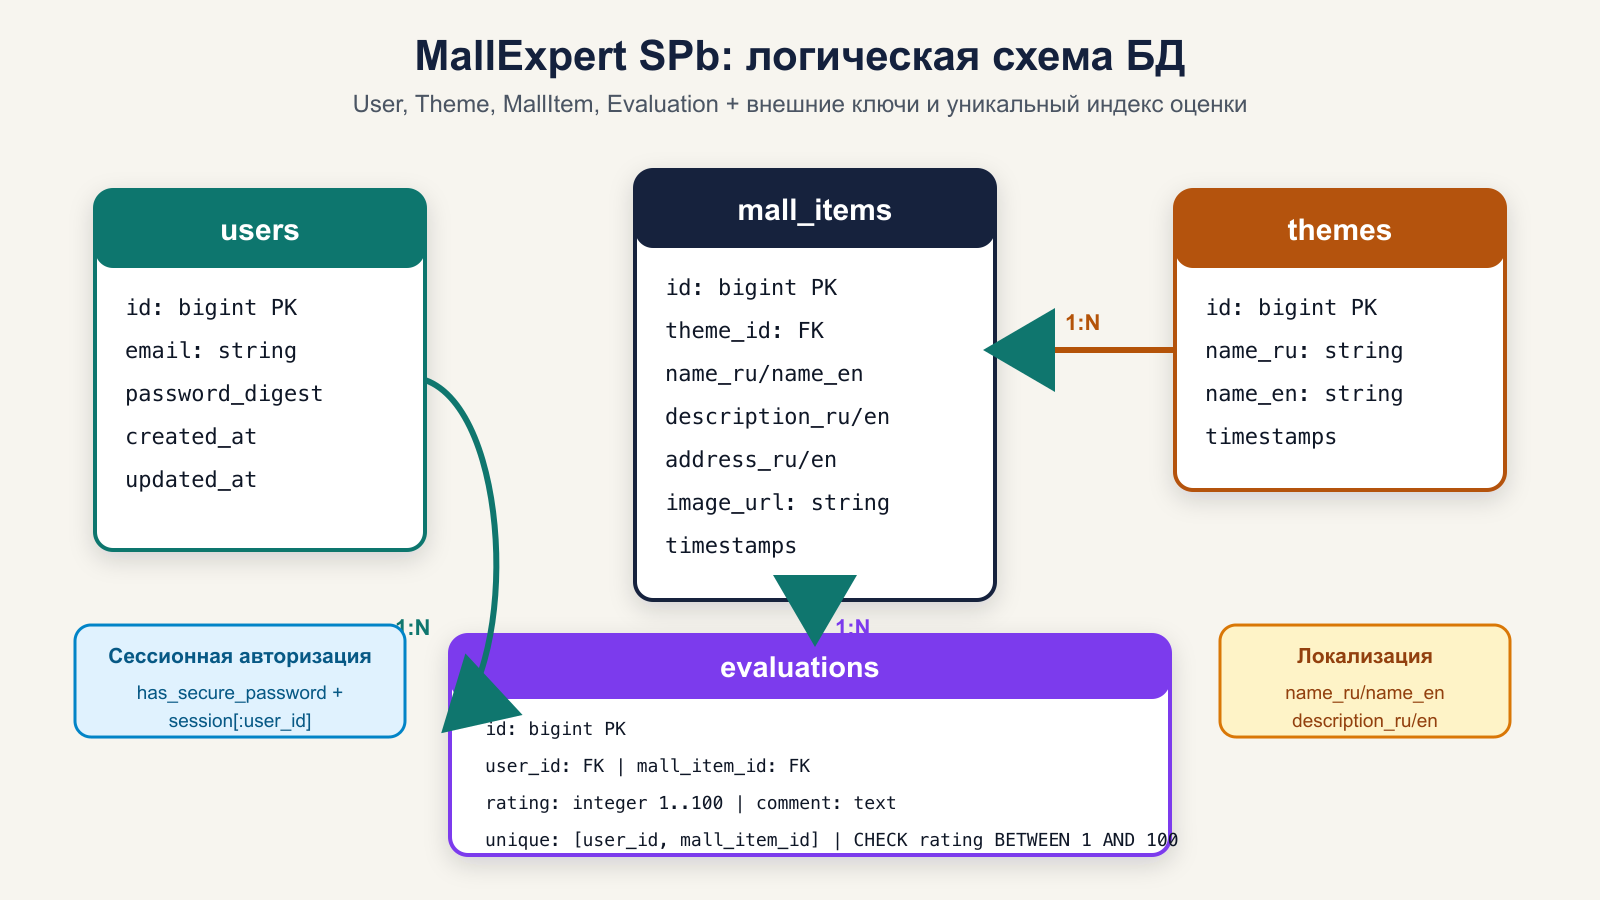
\includegraphics[width=\textwidth]{mall_schema_erd.png}
\caption{Разработанная мной логическая схема базы данных}
\end{figure}

\begin{figure}[H]
\centering
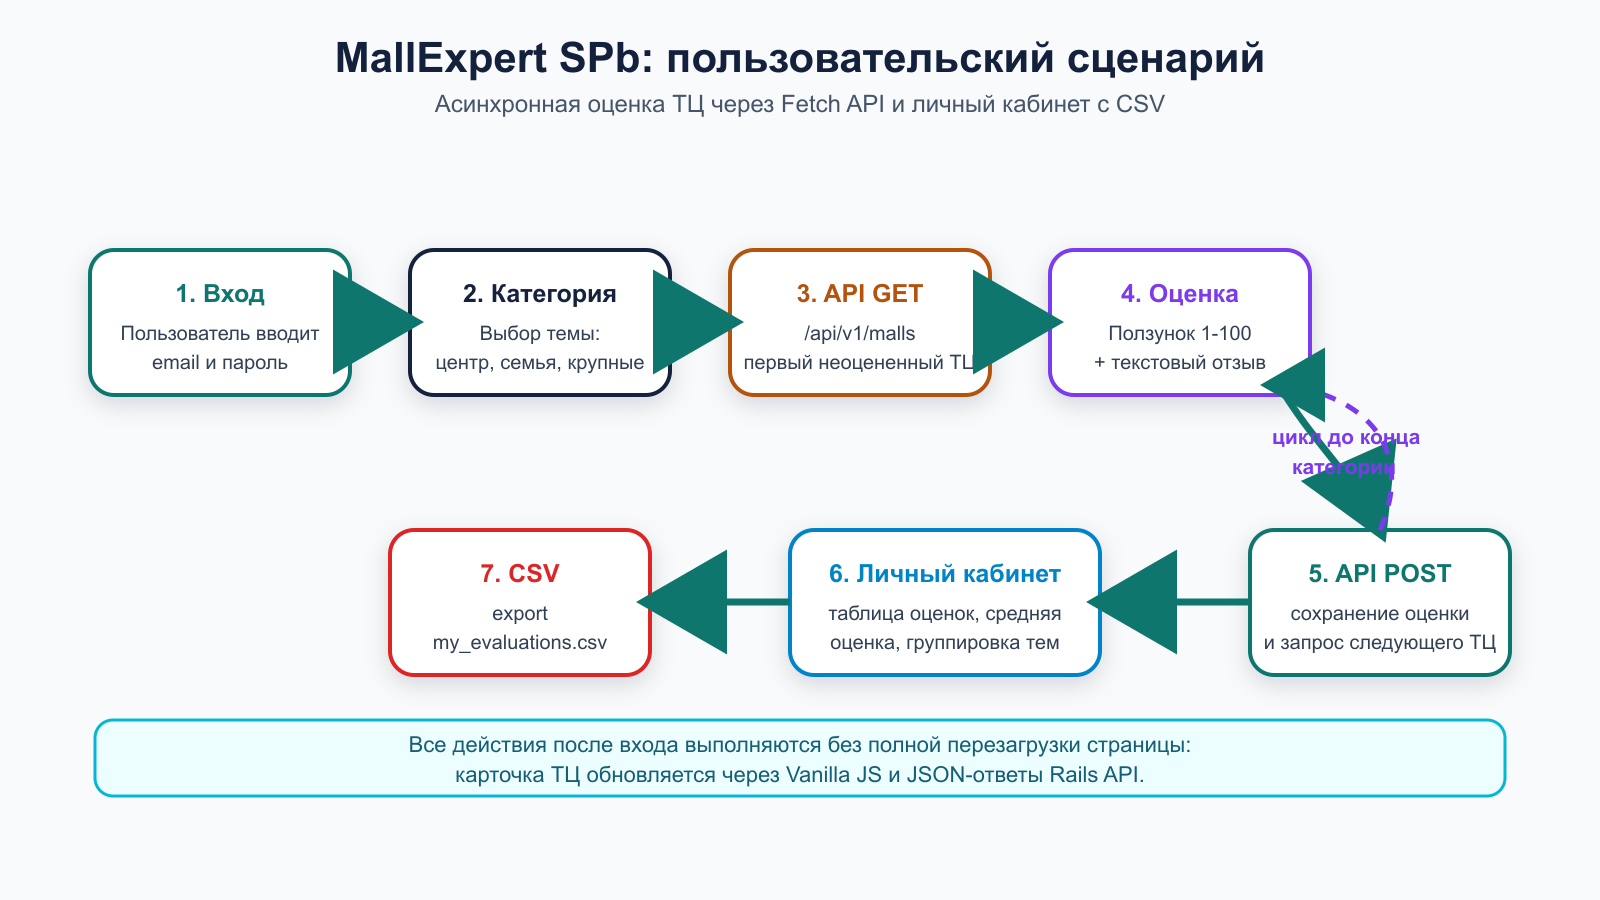
\includegraphics[width=\textwidth]{mall_flow.png}
\caption{Разработанный мной пользовательский сценарий оценки}
\end{figure}

\section{Реализация проекта}
\subsection{Кастомная сессионная авторизация}

В модели \texttt{User} я использовал \texttt{has\_secure\_password}. Для создания сессии я написал \texttt{SessionsController}: при успешной проверке пароля я сохраняю идентификатор пользователя в \texttt{session[:user\_id]}. В \texttt{ApplicationController} я реализовал методы \texttt{current\_user}, \texttt{logged\_in?} и \texttt{authorize}. Это позволило мне защитить рабочую область, личный кабинет и API.

\lstinputlisting[language=RubyCustom,caption={ApplicationController с локализацией и авторизацией}]{../app/controllers/application_controller.rb}

\subsection{Модель оценки и CSV}

В модели \texttt{Evaluation} я реализовал проверку диапазона 1--100, уникальность оценки и метод CSV-экспорта. Этот файл является центральным для бизнес-логики проекта.

\lstinputlisting[language=RubyCustom,caption={Модель Evaluation}]{../app/models/evaluation.rb}

\subsection{API и асинхронный обмен}

Метод \texttt{index} API получает тему и возвращает первый неоцененный ТЦ. Метод \texttt{create} сохраняет оценку, комментарий и возвращает JSON-статус. Я сделал API защищенным через \texttt{authorize}, поэтому неавторизованный пользователь не может сохранять оценки.

\lstinputlisting[language=RubyCustom,caption={API-контроллер оценки торговых центров}]{../app/controllers/api/v1/malls_api_controller.rb}

На клиентской стороне я написал JavaScript-файл, который загружает карточку, обновляет число рядом с ползунком, отправляет оценку и после сохранения запрашивает следующий ТЦ.

\lstinputlisting[language=JavaScriptCustom,caption={Клиентская логика Fetch API и ползунка 1--100}]{../app/javascript/malls_evaluation.js}

\subsection{Локализация}

В моем приложении локализованы и интерфейсные строки, и данные предметной области. В таблицах есть поля \texttt{name\_ru}, \texttt{name\_en}, \texttt{description\_ru}, \texttt{description\_en}, \texttt{address\_ru}, \texttt{address\_en}. Благодаря этому пользователь видит полноценную русскую или английскую версию карточки.

\subsection{Начальные данные}

В \texttt{db/seeds.rb} я создал три категории и десять реальных ТЦ Санкт-Петербурга: «Галерея», «Невский Центр», «Владимирский Пассаж», «Охта Молл», «Питерлэнд», «Гранд Каньон», «Европолис», «Лето», «Радуга», «Сити Молл». Также я добавил демо-пользователя \texttt{student@example.com}.

\section{Описание пользовательского интерфейса}

\begin{figure}[H]
\centering
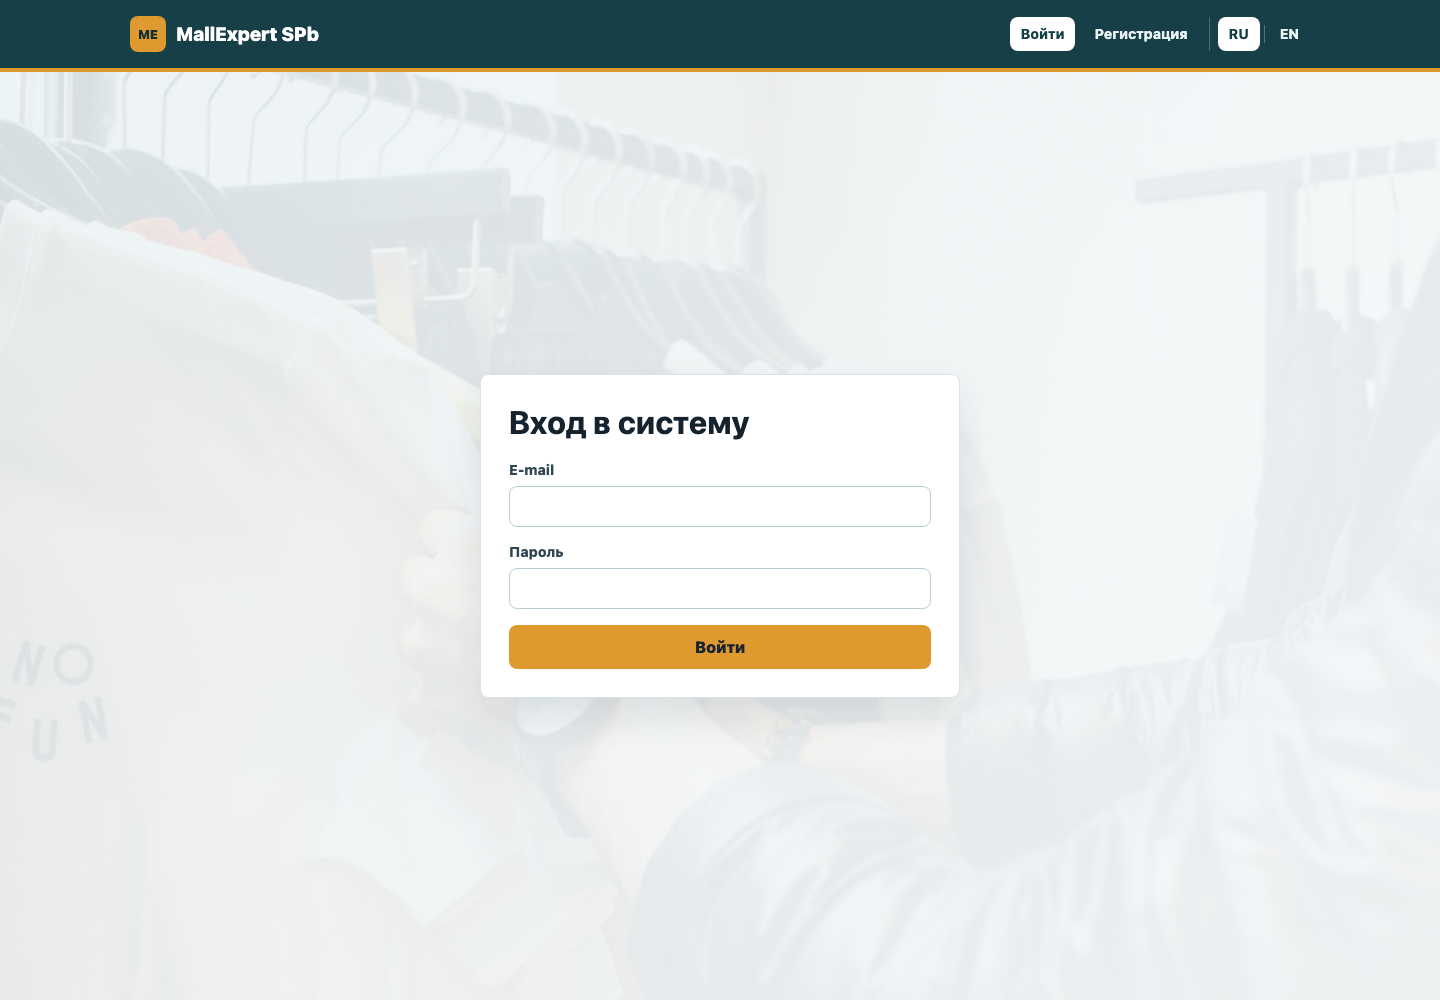
\includegraphics[width=\textwidth]{mall_login.png}
\caption{Страница входа в систему}
\end{figure}

\begin{figure}[H]
\centering
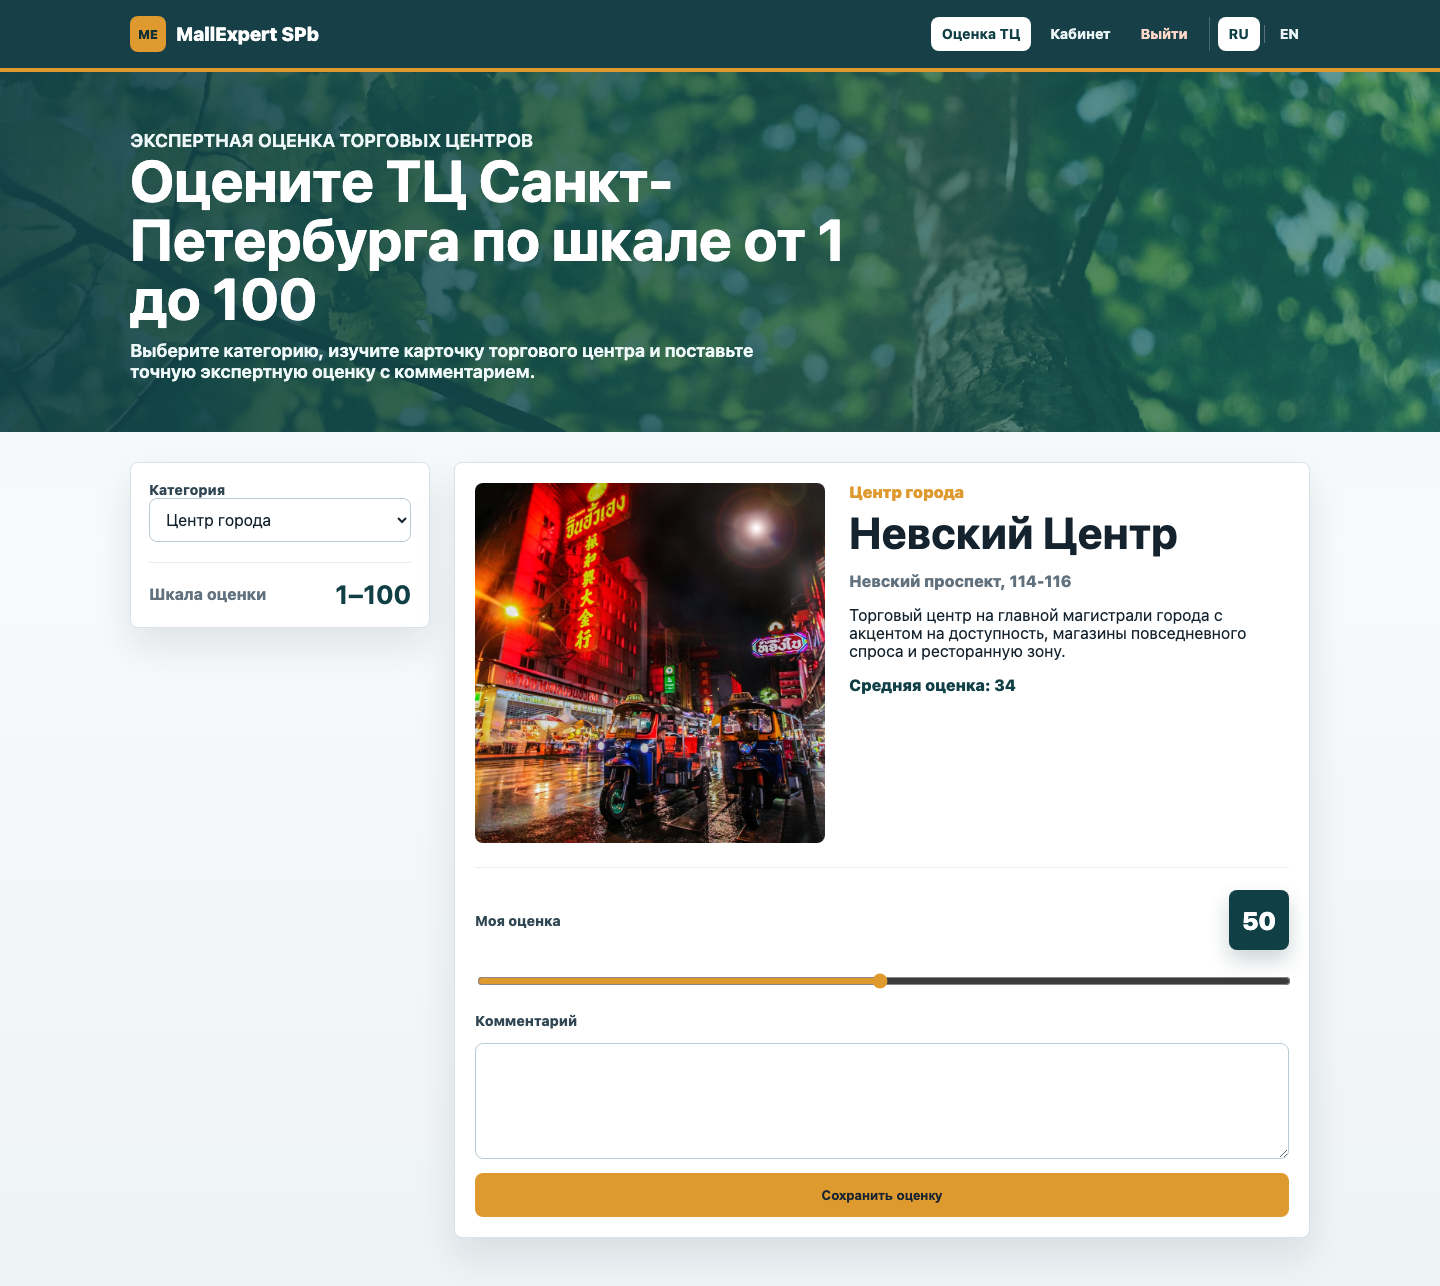
\includegraphics[width=\textwidth]{mall_work_ru.png}
\caption{Рабочая область оценки на русском языке}
\end{figure}

\begin{figure}[H]
\centering
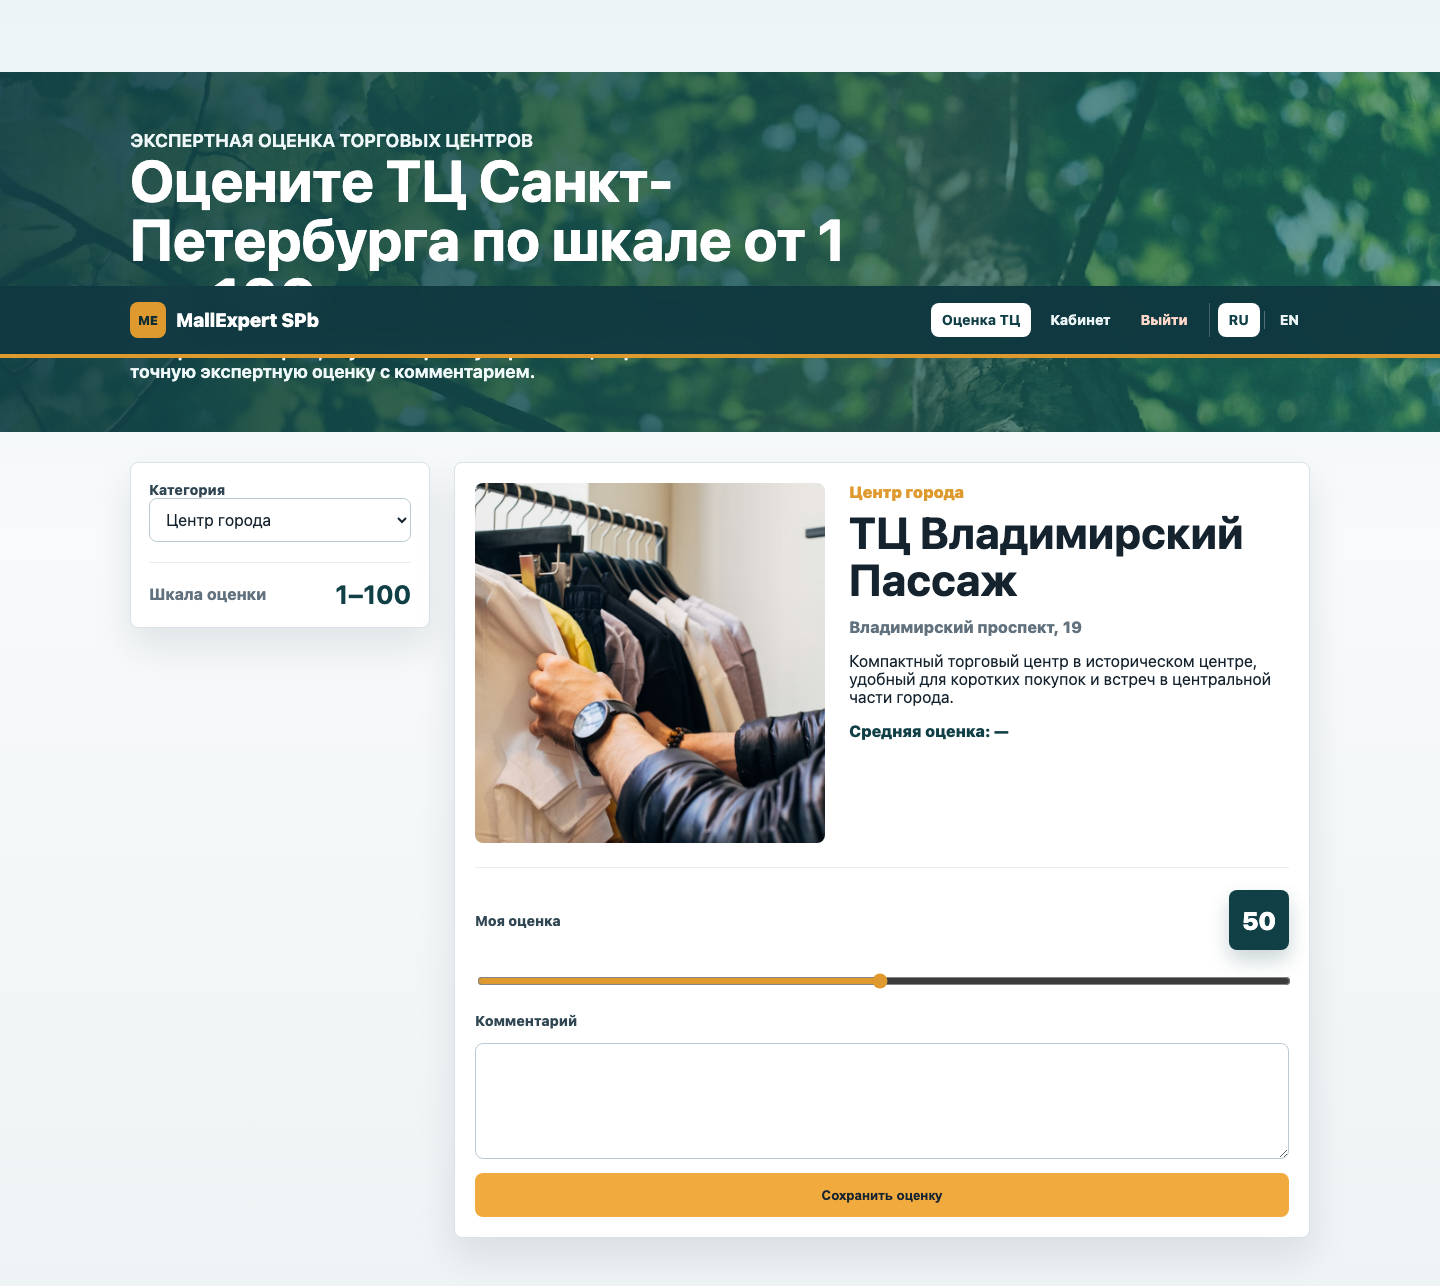
\includegraphics[width=\textwidth]{mall_after_rating.png}
\caption{Состояние интерфейса после сохранения оценки}
\end{figure}

\begin{figure}[H]
\centering
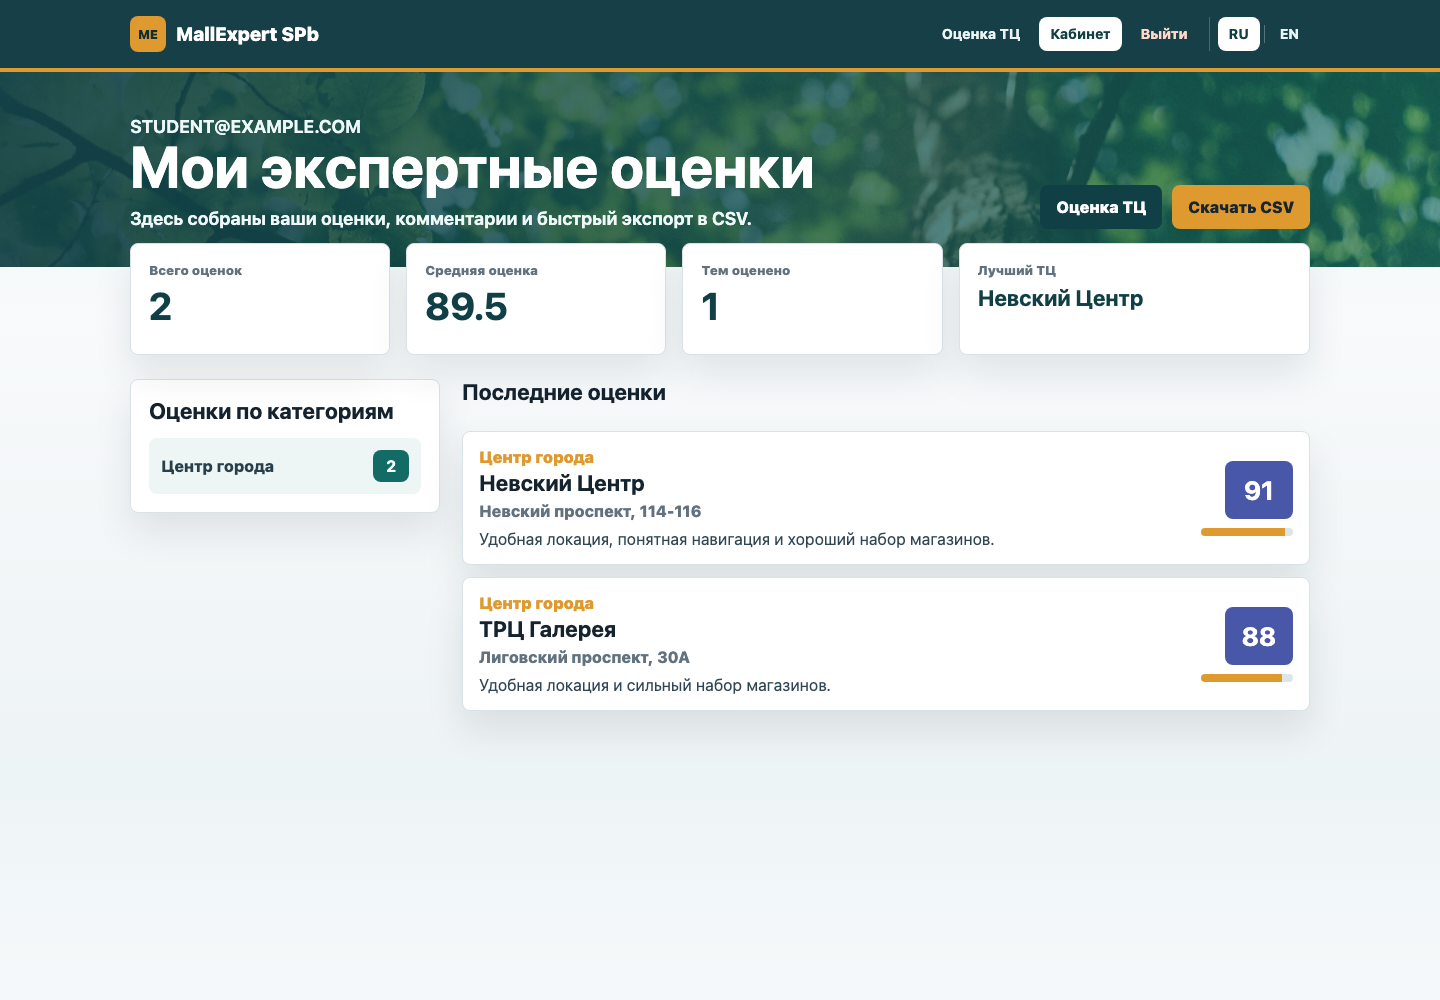
\includegraphics[width=\textwidth]{mall_profile.png}
\caption{Личный кабинет пользователя и CSV-экспорт}
\end{figure}

\begin{figure}[H]
\centering
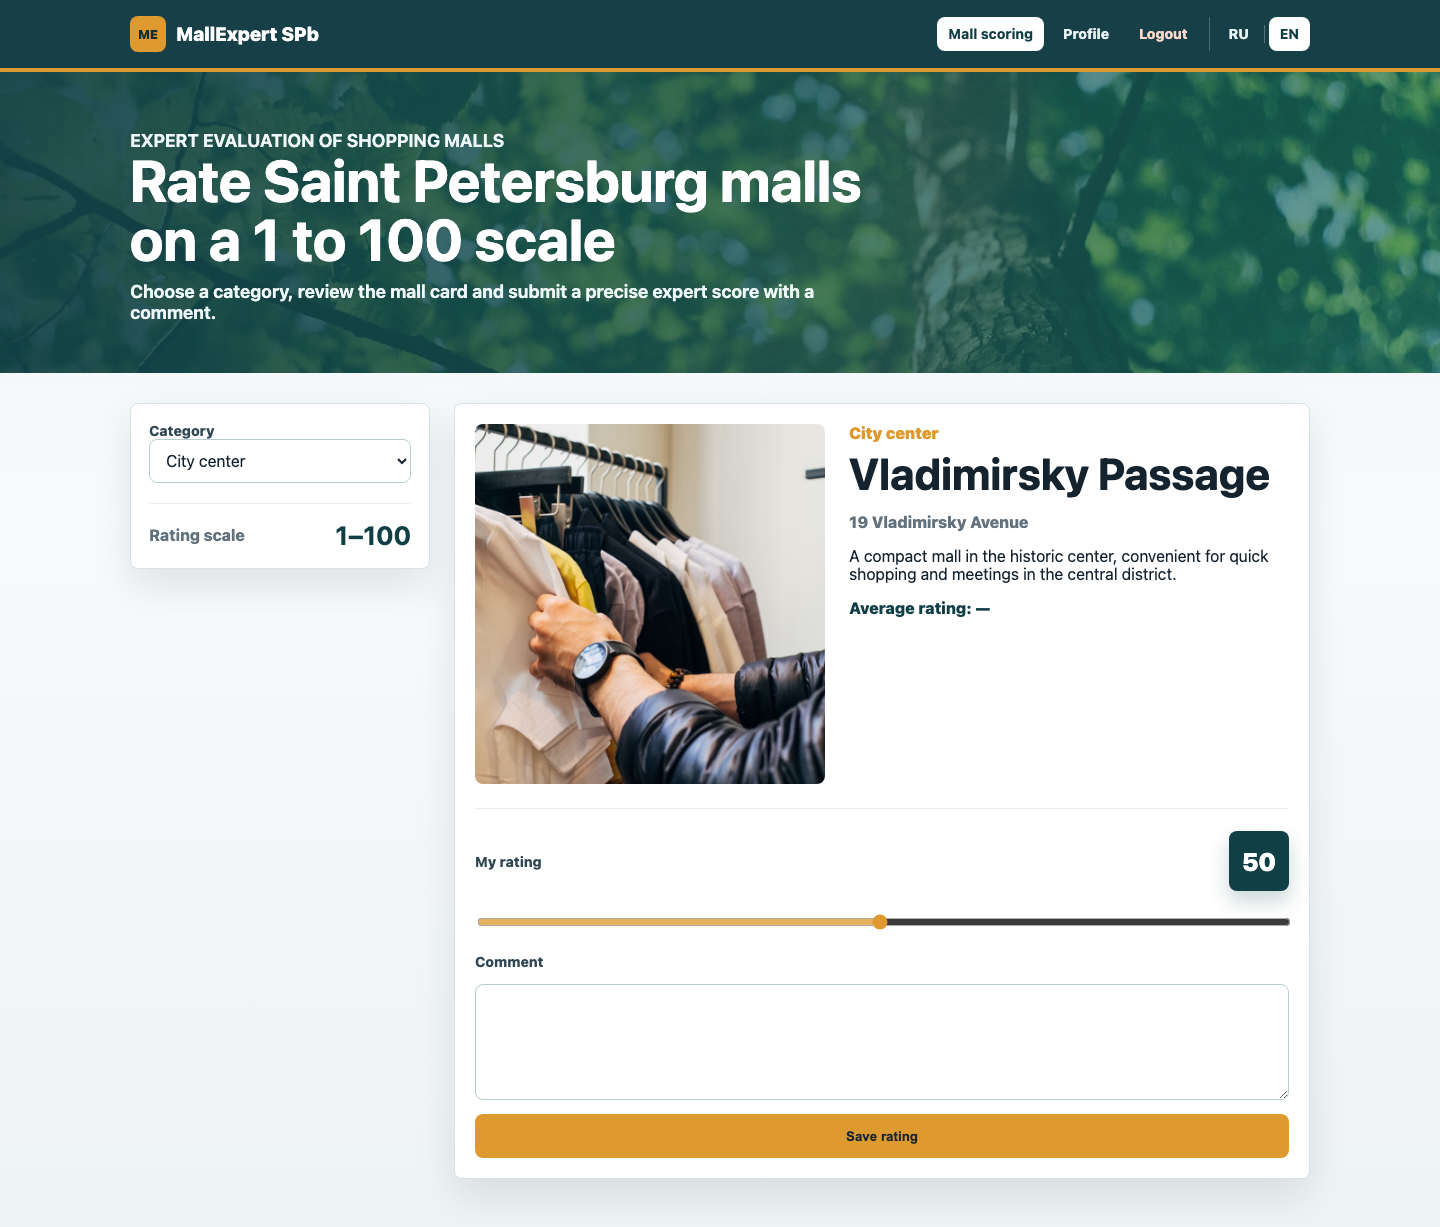
\includegraphics[width=\textwidth]{mall_work_en.png}
\caption{Английская локализация рабочей области}
\end{figure}

\section{Тестирование и отладка}

Я написал unit-тесты для моделей и integration-тест основного сценария. Unit-тесты проверяют диапазон оценки, уникальность пары пользователь-ТЦ, расчет средней оценки и CSV-экспорт. Интеграционный тест проверяет вход пользователя, открытие рабочей области, JSON-запрос карточки и сохранение оценки.

Smoke-test я выполнил вручную: открыл страницу входа, вошел под демо-пользователем, выбрал категорию, получил карточку, поставил оценку 88, написал комментарий, проверил переход к следующему объекту, открыл личный кабинет и переключил интерфейс на английский язык.

\section{Запуск проекта}

Локальный запуск:

\begin{lstlisting}[language=bash,caption={Команды локального запуска}]
cd /Users/doodels/.openclaw/workspace/projects/fooddecision-course
cp .env.example .env
bundle install
bin/rails db:create db:migrate db:seed
bin/rails server
\end{lstlisting}

Docker-запуск:

\begin{lstlisting}[language=bash,caption={Команды Docker-запуска}]
docker build -t mall-expert-course .
docker run --rm -p 3000:3000 \
  -e RAILS_ENV=development \
  -e POSTGRES_HOST=host.docker.internal \
  -e POSTGRES_USER=postgres \
  -e POSTGRES_PASSWORD=postgres \
  -e POSTGRES_DB=mall_expert_course_development \
  mall-expert-course \
  ./bin/rails server -b 0.0.0.0 -p 3000
\end{lstlisting}

\section{Результаты}

В результате я получил готовое WEB-приложение, которое соответствует требованиям промта. В нем реализованы Rails 8, PostgreSQL, ручная авторизация, модели предметной области, шкала 1--100, Fetch API, личный кабинет, CSV-экспорт, RU/EN-локализация, демо-данные и тесты. Проект можно открыть по адресу \texttt{http://localhost:3000/ru}.

\section{Заключение}

В ходе курсового проекта я разработал полноценное Rails-приложение от структуры базы данных до пользовательского интерфейса и отчета. Для меня главным результатом стала связка серверной MVC-логики и асинхронного клиентского сценария. Rails 8 позволил быстро собрать основу приложения, но при этом я явно контролировал авторизацию, маршруты, ограничения данных, локализацию и формат API.

Я считаю итоговую версию MallExpert SPb готовой к сдаче: она запускается, содержит тесты, имеет демонстрационные данные и сопровождается пояснительной запиской со скриншотами и листингами.

\section{Список использованных источников}

\begin{enumerate}
  \item Ruby on Rails Guides. URL: \url{https://guides.rubyonrails.org/}
  \item Ruby on Rails API Documentation. URL: \url{https://api.rubyonrails.org/}
  \item PostgreSQL Documentation. URL: \url{https://www.postgresql.org/docs/}
  \item Ruby CSV Documentation. URL: \url{https://ruby-doc.org/stdlib/libdoc/csv/rdoc/CSV.html}
  \item MDN Web Docs: Fetch API. URL: \url{https://developer.mozilla.org/en-US/docs/Web/API/Fetch_API}
  \item MDN Web Docs: HTML input range. URL: \url{https://developer.mozilla.org/en-US/docs/Web/HTML/Element/input/range}
  \item Rails Internationalization Guide. URL: \url{https://guides.rubyonrails.org/i18n.html}
  \item Docker Documentation. URL: \url{https://docs.docker.com/}
\end{enumerate}

\appendix
\section{Приложение. Дополнительные листинги}

\lstinputlisting[language=RubyCustom,caption={Gemfile проекта}]{../Gemfile}
\lstinputlisting[language=RubyCustom,caption={Модель MallItem}]{../app/models/mall_item.rb}
\lstinputlisting[language=RubyCustom,caption={ProfilesController}]{../app/controllers/profiles_controller.rb}
\lstinputlisting[language=RubyCustom,caption={Интеграционный тест пользовательского сценария}]{../test/integration/mall_workflow_test.rb}

\end{document}
